\chapter{Nově navržený systém}
\label{Nově navržený systém}
%V této kapitole se budem zabívat nově navrženým systémem, jejíma komponentama a... 
Nově navržený systém se skládá z databáze a 5 hlavních komponent navzájem propojených: mikrokontrolér, váha, čtečka čárového kódu, displej a klávesnice. Dále je možnost připojit systém k počítači pro správu databáze a tisk dat. 

\section{Postup měření}%/Princip/funkcionalita
Pro evidenci zůstatkového objemu jedné láhve je nutné naskenovat její čárový kód pomocí čtečky čárových kódů a zvážit ji. Mikrokontroler na základě získaného EAN vybere z databáze patřičná data, viz kapitola č. \ref{databaze} a přepočítá hmotnost na objem. V případě, že by čárový kód nebyl čitelný, je možné ho zadat ručně do systému prostřednictvím klávesnice. Veškeré důležité informace včetně zbytkového objemu se zobrazí na displeji. %Pro výpis všech naměřených dat je možné systém připojit k počítači a nechat si je vytisknout do formátu .xlsx pomocí navržené desktopové aplikace. Tato aplikace slouží i ke správě databáze.
%Do budoucna k měřicimu systému bude vyvíjena desktopová aplikace běžící na stolním počítačí/notebooku. Mikrokontroler bude k počítači připojen prostřednictvím USB portu
%Do budoucna pro výpis všech naměřených dat bude možné systém připojit k počítači a nechat si je vytisknout do formátu  .xlsx pomocí navržené desktopové aplikace. Tato aplikace slouží i ke správě databáze.

Do budoucna bude vyvíjena desktopová aplikace pro editaci databáze[č.5.3] a zpracování naměřených dat, jako je například tisk do formátu .xlsl. Měřící systém bude propojený s počítačem skrz USB kabel nebo Wi-Fi.

\section{Blokové schéma}
%FOTO
%Výpočetní jednotka Raspberry pi pracuje s databázi dat jednotlivých destilátů. V první řadě je nutné tuhle databází vytvořit a implementovat prostřednictvím desktopové aplikace. 
\begin{figure}[!h]
    \begin{center}
        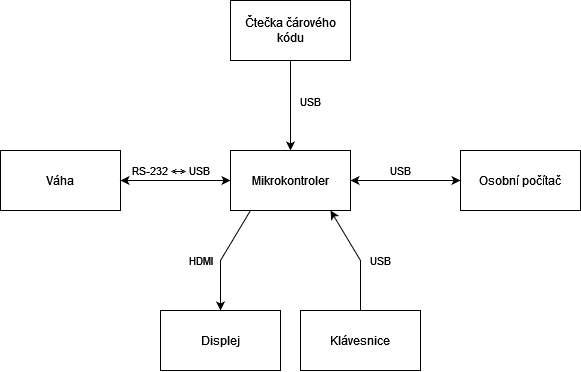
\includegraphics[scale=0.7]{obrazky/Blokové schéma.png}
    \end{center}
    \label{blokove_schema}
    \caption{Blokové schéma nově navrženého systému}
\end{figure}

\section{Databáze}
\label{databaze}
%Celý systém je závislý na datech, které nesou informace o názvu destilátu
Aby bylo možné přepočítat hmotnost na objem je nutné znát předem hmotnost prázdné a plné láhve a její maximální objem. Postup výpočtu je zmíněn v kapitole č. \ref{odkazos}. Tyto data jsou uloženy v relační\footnote{Data uložený v tabulkách, kde sloupce reprezentují atributy a řádky jednotlivé záznamy, řádky jsou propojeny pomocí tzv. klíčů. Tabulky \ref{databaze_destilatu} a \ref{tab:my_label} mají prohozené řádky a sloupce z důvodu lepšího umístění na stránku.} databázi včetně informací jako jsou: název destilátu, EAN kód, maximální objem, nebo adresa k obrázku daného produktu.
%K datům se přistupuje pomocí EAN kódu nebo názvem destilátu zadaný klávesnicí.

%Některé destiláty, mají na svém hrdle nalévač místo vršku, který mění hmotnost láhve. Aby naš systém byl časově efektivní, tak implementujeme druhou databázi 

%Některé destiláty mají na svém hrdle nalévátko (obrázek č. \ref{nalevačos}) místo víčka, který mění hmotnost láhve. V takovém případě bychom museli nalévač nahradit víčkem, aby hmotnost láhve odpovídala předpisu funkce, což je časově neefektivní. Místo toho byla navržena druhá databáze, obsahující hmotnosti různých nalévačů. Vzorec pro výpočet objemu ve výchozím nastavení počítá s víčkem na láhvi, proto uživatel musí při měření zakliknout pomocí klávesnice, že chce měřit objem s nalévačem. Při výpočtu dojde k nahrazení hmotnosti víčka hmotností nalévače a následně dojde k výpočtu výsledného objemu.

Některé destiláty mají na svém hrdle nalévač nebo také nalévátko (obrázek č. \ref{nalevačos}) místo víčka, který mění hmotnost láhve. V takovém případě bychom museli nalévač nahradit víčkem, aby hmotnost láhve odpovídala předpisu rovnice č.xyz (skutečná hmotnost prázdné láhve musí odpovídat s hodnotou hmotnosti prázdné láhve v databázi), což je časově neefektivní. Místo toho byla navržena druhá databáze, obsahující hmotnosti různých nalévačů. Vzorec pro výpočet objemu ve výchozím nastavení počítá s víčkem na láhvi, proto uživatel musí při měření zakliknout v aplikaci, že chce měřit objem s nalévačem. Při výpočtu dojde k nahrazení hmotnosti víčka hmotností nalévače a následně dojde k výpočtu výsledného objemu.


%Vyhledání destilátu a jeho dat je porstřednictvím EAN kódu nebo jeho názvu.

Obě databáze jsou uložené v mikrokontroléru.

%FOTO
\begin{table}[!h]
\centering
\begin{tabular}{|l|l|l|l|}
\hline
 & Destilát č. 1   & Destilát č. 2   &  . . . \\ \hline
\textbf{Název destilátu} [-] [\textit{TEXT}] &   &    &  \\ \hline
\textbf{EAN kód} [-] [\textit{INTEGER}]&  &    &        \\ \hline
\textbf{Hmotnost prázdné láhve} [g] [\textit{numeric}] &    &  &        \\ \hline
\textbf{Hmotnost plné láhve} [g] [\textit{numeric}] &    &    &  \\ \hline
\textbf{Hmotnost víčka} [g] [\textit{numeric}] &    &    &  \\ \hline
\textbf{Maximální objem láhve} [l] [\textit{numeric}] &    &    &  \\ \hline
\textbf{Množství alkoholu} [\%] [\textit{numeric}] &    &    &  \\ \hline
\textbf{Adresa obrázku} [-] [\textit{TEXT}] &    &    &  \\ \hline
%Obrázek: obsahuje adresu/název obrázku, který je uložen ve složce
\end{tabular}
\label{databaze_destilatu}
\caption{Databáze destilátů}
\end{table}


\begin{table} [!h]
    \centering
    \begin{tabular}{|l|l|l|l|}
    \hline
         & Nalévač č. 1 & Nalévač č. 2 &  . . .\\ \hline
         \textbf{Název nalévače} [-] [\textit{TEXT}] & & &\\ \hline
         \textbf{Výrobce} [-] [\textit{TEXT}] & & &\\ \hline
         \textbf{Hmotnost} [g] [\textit{numeric}] & & &\\ \hline
         \textbf{Adresa obrázku} [-] [\textit{TEXT}] & & &\\ \hline
    \end{tabular}
    \caption{Databáze nalévačů}
    \label{tab:my_label}
\end{table}

\begin{figure}[!h]
    \begin{center}
        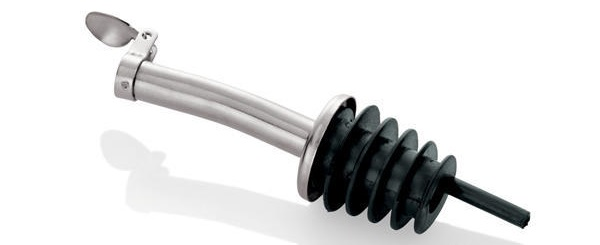
\includegraphics[scale=0.6]{obrazky/nalevac.jpg}
    \end{center}
    \label{nalevačos}
    \caption{Nalévač na alkohol \cite{nalevatko}}
\end{figure}
% \definecolor{Silver}{rgb}{0.752,0.752,0.752}
% \begin{table}[!h]
%     \centering
%     \begin{tabular}
%         {
%         cell{1}{4} = {c},
%         hlines = {Silver},
%         vlines = {Silver},
%         }
%         Název & hmotnost\\
%         Nalévač č.1 & x\\
%     \end{tabular}
%     \caption{Caption}
%     \label{tab:my_label}
% \end{table}
%\usepackage{color}
%\usepackage{tabularray}
%\definecolor{Silver}{rgb}{0.752,0.752,0.752}
%\begin{tabular}[
%  label = none,
%  entry = none,
%]{
%  cell{1}{4} = {c},
%  hlines = {Silver},
%  vlines = {Silver},
%}
%Název destilátu & destilát č.1 & destilát č.2 & . . . \\
%EAN kód & & & \\
%hmotnost prázdné láhve & & & \\
%hmotnost plné láhve    &              & & \\
%hmotnost víčka         &              &              &       \\
%obrázek                &              &              &       \\
%max. objem             &              &              &       
%\end{tabular}
%Tabulka destilátů
%Nazev | EAN | k | q | m_víčko | max_objem | obrazek | poznamka
%Tabulka druhů nalévačů
%Nazev | m_nalevač | obrazek

\section{Váha}

Nejdůležitější komponentou systému je váha pro výpočet zbytkového objemu z naměřené hmotnosti láhve, viz kapitola č.\ref{Přepočet hmotnosti na objem}.  Proto v této podkapitole rozeberu požadavky, výběr váhy a její alternativy.
%
%Váhy jsou zařízení, která slouží k měření hmotnosti objektů. Existuje mnoho typů vah, ale základní princip je stejný. Váhy se skládají ze dvou hlavních částí: měřicího mechanismu a zobrazovacího mechanismu.
%
%Měřicí mechanismus se skládá z vážícího tělesa a pružiny. Když položíte objekt na váhu, pružina se stlačí a vážící těleso se posune dolů. Tento pohyb se přenáší na měřicí stupnici, která ukazuje hmotnost objektu.
%
%Zobrazovací mechanismus se skládá z displeje a elektronického obvodu. Elektronický obvod přijímá signál od měřicího mechanismu a převádí ho na čitelný formát pro displej. Displej pak zobrazuje hmotnost objektu.[zdroj]
%
%\subsection{Elektronická část váhy}
%
%Elektronická část váhy se skládá z senzoru a elektronického obvodu. Senzor měří deformaci, kterou způsobuje vážený objekt, a převádí ji na elektrický signál. Tento signál je poté zpracován elektronickým obvodem, který obsahuje A/D převodník a mikroprocesor.
%
%Senzory používané v elektronických vahách jsou obvykle tenzometry nebo load cells. Tenzometry jsou malé senzory, které měří změnu odporu, když jsou deformovány. Load cells jsou senzory, které měří změnu napětí, když jsou deformovány. Oba typy senzorů jsou velmi přesné a umožňují měření hmotnosti s vysokou přesností.
%
%A/D převodník převádí analogový signál z senzoru na digitální signál, který může být zpracován mikroprocesorem. Mikroprocesor pak zpracovává signál a zobrazuje výslednou hmotnost na displeji. [zdroj]
%
\subsection{Požadavky na váhu}

Hlavním požadavkem je oboustranný otevřený komunikační port pro čtení dat a odesílání požadavku na jejich zaslání prostřednictvím sériové linky do řídící jednotky, je tedy nutné znát přesný popis přenosu dat. Tyto požadavky zpravidla splňují laboratorní a průmyslové váhy, kde se očekává, že data budou zpracovávána pomocí aplikačního softwaru.

Váživost (maximální hmotnost, která lze na váze navážit) se požaduje minimálně 2 kg. Hmotnost prázdné láhve u většiny destilátů se pohybuje od 500 do 800 g a samotný obsah láhve je od 500 do 1000 ml, tudíž až necelý 1 kg. V případě robustnějších lahví okolo 1 kg by váživost do 2 kg nemusela stačit, proto je vhodnější volit 3 kg. Větší váživost jak 3 kg, by neměla pro běžné podniky HoReCa význam, navíc s vyšší váživostí úměrně klesá její přesnost a roste cena váhy.

Přesnost, jinak řečeno rozlišení nebo odčitatelnost, se udává v dílcích(d). Dílek je nejmenší hodnota hmotnosti, kterou lze z displeje váhy odečíst.\cite{vazivost} Měření zbytkového objemu destilátu při inventurách není záležitostí "laboratorního měření" a zákon nestanovuje s jakou přesností je nutné měřit objem v láhvích pro inventurní účely. Obecně na 
přesnost není kladen velký důraz. Tím, že žádná norma nestanovuje, jakou přesnost by měl mít nově navržený měřicí systém, by bylo optimální, aby měřilo s přesností stejnou nebo vyšší než odměrné válce. Odměrné válce na alkohol
(kapitola č. \ref{valec_na_alkohol}) mají přesnost ±5 ml. Obyčejné odměrné válce (kapitola č. \ref{obecny_valec}) třídy B mají přesnost ±10 ml a třídy A ±5 ml.

Požadovaná přesnost váhy závisí na hustotě měřené kapaliny.  Čím hustší kapalinu máme, tím menší přesnost vyžadujeme, a naopak - méně hustá kapalina bude vážit méně na jednotku objemu, v našem případě 10 ml. Tudíž nás zajímá, která složka destilátu má nejmenší hustotu. Ve své podstatě bude měřen pouze ethanol a voda, co se týče příměsí pro dochucení, tak ty jsou větší hustoty, proto přesnost váhy vztáhneme k ethanolu, i když nikdy nebudeme měřit 100\% ethanol, ale jeho směs s vodou a dalšími příměsi. Požadovaná přesnost váhy tedy je ±3,95 g (10 ml ethanolu), postup výpočtu níže[\ref{presnost vahy}]:\\

Výpočet přesností váhy:
%\begin{equation}
%    Presnost\, váhy = \frac{V_{max}-V_{min}}{m_{max}-m_{min}}\, \left[\mathrm{m^3/kg}\right]\label{presnost vahy}
%\end{equation}

%\begin{equation}
%    Přesnost\ váhy = Přesnost\ válce \cdot Hustota\ kapaliny \label{presnost vahy}
%\end{equation}

\begin{equation}
    %U(m) = U(V) \cdot \rho 
    \Delta m = \Delta V \cdot \rho \label{presnost vahy}
\end{equation}

\(\Delta m\) ...Přesnost váhy \([\mathrm{g}]\) %Nejistota hmotnosti (přesnost váhy)

\(\Delta V\) ...Přesnost válce \([\mathrm{ml}]\) %...Nejistota objemu (přesnost válce)

\(\rho\) ...Hustota nejlehčí složky destilátu (ethanol) \([\mathrm{g/ml}]\)

\begin{equation}
    \Delta m = \pm5 \cdot 0,79 = \pm3,95 \, \left[\mathrm{g}\right] \label{presnost vahy}
\end{equation}



Váha je určena pro fyzickou inventuru HoReCa podniků, která spadá pod interní činnost podniku a není podmínkou, aby byla certifikována viz. kapitola č.\ref{meridlo}
%Váha je určena pro interní chod podniku a není podmínkou, aby byla certifikována.

Po splnění výše zmíněných požadavků je rozhodujícím faktorem cena.
\\ \\
%zdroj: https://www.hepnar.cz/poradna/view/co-je-to-max-vazivost-a-dilek/
%Posledním parametrem je cena, kdy
%Váha by měla být kompaktní, aby ji bylo možné
%Při inventurách je hlavním problémem časová náročnost a 
%Přesnost v našem případě není až tak důležitou vlastností
\textbf{Souhrn požadavků prioritně seřazených:} %sestupně / 
\begin{itemize}
    \item Oboustranný otevřený komunikační port
    \item Váživost nad 2 kg
    \item Přesnost ±3,95 g a více
    \item Nízká cena
\end{itemize}

\subsection{Vybraná váha}
%Při výběru váhy jsem se řídil výše zmíněnými požadavky, kdy. 

Váha byla vybrána na základě výše zmíněných požadavků.
Základní parametry váhy jsou vyobrazené v tab. č \ref{vahaa}.
%Kompletní dokumentace je v příloze č. x
Kompletní specifikace je uvedena v dokumentaci: \cite{vaha_datasheed}



\begin{table}[!h]
    \centering
    \begin{tabular}{|c|c|}
        \hline
        Výrobce                                                         & G\&G   \\ \hline
        Model                                                           & E3000  \\ \hline
        %\begin{tabular}[c]{@{}c@{}}Komunikační\\ protokol\end{tabular}  & UART   \\ \hline
        \begin{tabular}[c]{@{}c@{}}Komunikační \\ rozhraní\end{tabular} & RS-232 \\ \hline
        \begin{tabular}[c]{@{}c@{}}Datový \\ konektor\end{tabular} & \begin{tabular}[c]{@{}c@{}}DE-9\\ (Samice)\end{tabular} \\ \hline
        Váživost                                                        & 3 kg    \\ \hline
        Přesnost                                                        & 0.5 g     \\ \hline
        \begin{tabular}[c]{@{}c@{}}Doba \\ stabilizace\end{tabular} & < 2 s \\ \hline
        Cena                                                            & 1987 Kč     \\ \hline
    \end{tabular}
    \label{vahaa}
    \caption{Základní parametry vybrané váhy}
\end{table}

\begin{figure}[!h]
    \begin{center}
        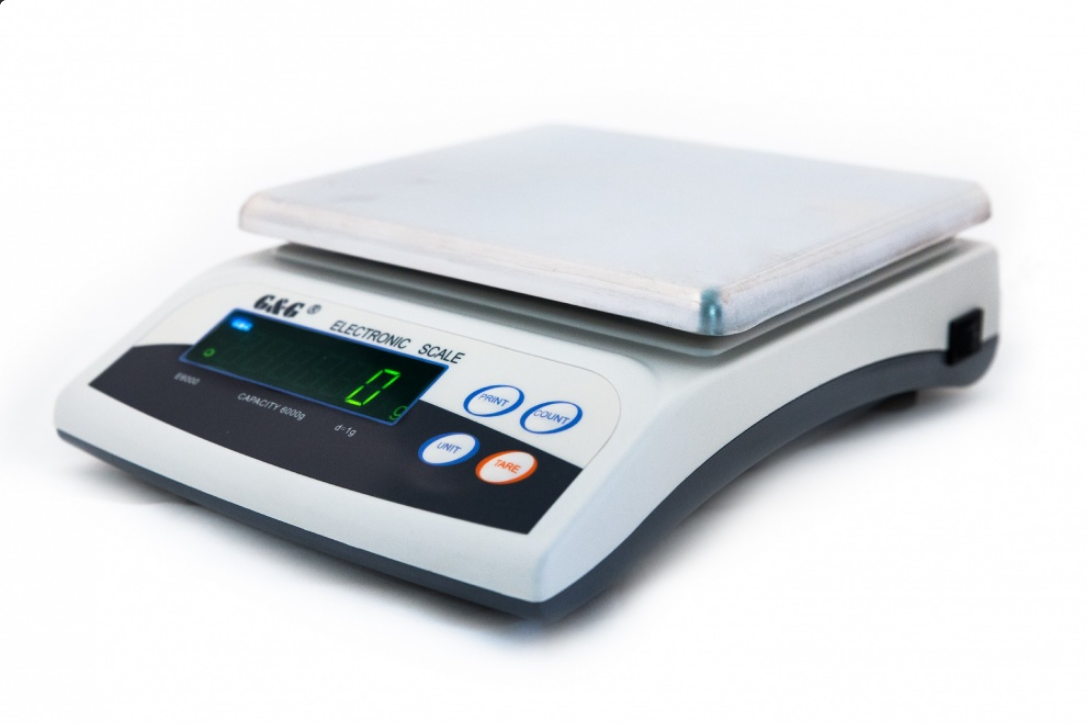
\includegraphics[scale=0.25]{obrazky/E3000.png}
    \end{center}
    \caption{Vybraná váha G\&G E3000 \cite{vaha}}
\end{figure}



% Jeden z hlavních požadavků bylo, aby váha obsahovala otevřený oboustranný komunikační port, jak pro čtení dat, tak i pro odesílání požadavků pro tisk.
% Zvolena váha disponuje RS-232 portem s komunikačním protokolem UART.

% Váživost byla volena 3Kg, protože většina větších destilátů váží do 2kg. Tudíž máme 1kg rezervu.

% Přesnost v našem případě nehraje, až tak významnou roli, proto byla váha vybírána na základě poměr "cena/výkon". Přesnost činní 0,5g.

%\subsection{Datový přenos}

%Váha posílá data přes RS-232 rozhraní. viz. kapitola č.x. Díky výstupnímu napětí 5V je možné bez nutnosti napěťového děliče připojit váhu přímo na vstup mikrokontroleru. Bohužel raspbery pi 4 disponuje pouze jedním UART rozhraním, který funguje v topologii pear-to-pear a bylo vyhrazeno pro senzor čárového kódu. Váha je tedy připojena na USB port, díky redukci RS-232 na USB, kdy propojení pinů je následovný:
%\begin{itemize}
%    \item Tx -> -D
%    \item Rx -> +D
%   \item COM -> COM
%\end{itemize}
%Napěťový vodič je pro náš systém zbytečný, proto není uvažován a datový vodiče jsou zapojený do kříže z důvodu pear-to-pear topologie.

\subsection{Datový paket}
\label{datový paket váhy}

Paket se skládá z:
\begin{itemize}
    \item 1 start bit
    \item 8 datových bitů
    \item 1 stop bit
    \item bez paritního bitu
\end{itemize}
%V našem případě není vyžadován paritní bit z důvodu opětovného odesílání stejných dat na výstup. Přínos by mohl mít pokud bychom ukládali veškeré příchozí data. Systém vezneme pouze poslední příchozí hodnotu, pokud sekvence dat za touhle hodnotou byla neměnná(např. za ±1 sekundu), tedy že se nám ustálila naměřená hmotnost.
%
%Datový paket váhy neobsahuje paritní bit, tudíž není možné zjistit zda zpráva není poškozena. Ošetření absence paritního bitu bude na SW úrovni. Pokud váha bude stabilizovaná a poslední 3 přijaté zprávy budou shodné, můžeme tuto hodnotu prohlásit/brát jako validní/správnou (nepoškozenou).
Datový paket váhy neobsahuje paritní bit, tudíž odhalení poškozené zprávy je obtížnější. Ošetření absence paritního bitu bude na softwarové úrovni, kdy se vyhodnotí poslední 3 přijaté zprávy, pokud budou všechny shodné, můžeme prohlásit, že tato hodnota je s největší pravděpodobností nepoškozená. Pravděpodobnost, že by 3x po sobě přišla stejně poškozená zpráva, je vysoce mizivá.

%Datový paket váhy neobsahuje paritní bit, což ztěžuje detekci případného poškození zprávy. Absence paritního bitu bude proto řešena na softwarové úrovni: vyhodnotí se poslední tři přijaté zprávy a pokud se všechny shodují, lze předpokládat, že jsou pravděpodobně nepoškozené. Pravděpodobnost trojnásobného opakovaného poškození stejné hodnoty je totiž téměř zanedbatelná.
%Další varianty textu: https://chatgpt.com/c/67c9adf8-0744-8000-a2f2-0d6be1335475



%\subsection{Datový rámec} %datový formát

%Datový rámec je část paketu, který obsahuje informace o hmotnosti viz. kapitola č.\ref{UARTt}. Dle dokumentace se formát skládá ze 14 bajtů zakódovaný v ASCII. Na obrázku č.\ref{data} je vidět posloupnost bajtů a jejich význam a na obrázku č.\ref{priklad} je praktický příklad.

%Datový rámec je část paketu, který obsahuje informace o hmotnosti viz. kapitola č.\ref{UARTt}. Dle dokumentace se formát skládá ze 14 bajtů zakódovaný v ASCII. Na obrázku č.\ref{data} je vidět posloupnost bajtů a jejich význam a na obrázku č.\ref{priklad} je praktický příklad.

Předpis výstupních dat se nachází v tabulce. \ref{tabos}, kdy dle dokumentace se formát skládá ze 14 bajtů zakódovaných v ASCII. V tabulce č. \ref{jouu} je praktický příklad.

%\begin{figure}[!h]
%    \begin{center}
%        \includegraphics[scale=0.5]{obrazky/data protokol - váha.PNG}
%    \end{center}
%    \label{data}
%    \caption{Předpis výstupních dat (1 unit = 1 bajt) \cite{vaha_datasheed}}
%\end{figure}

\begin{table} [!h]
    \centering
    \begin{tabular}{|l|l|l|l|l|l|}
    \hline
         Znaménko    & Mezera & Data &  Jednotka & Enter & Posun řádku \\ \hline
         1 B & 1 B           & 7 B           & 3 B &1 B&1 B\\ \hline
    \end{tabular}
    \caption{Předpis výstupních dat}
    \label{tabos}
\end{table}

%\begin{itemize}
%    \item space - "prázdný bit" %pro zachování velikosti 14-bitového slova
%    \item enter - přesunutí na začátek řádku (značení CR v ASCII: $\backslash$r)
%    \item linefeed - odřádkování (značeno LF, v ASCII: $\backslash$n) 
%\end{itemize}




\begin{table}[h]
\centering
\begin{tabular}{|p{0.6cm}|p{0.6cm}|p{0.6cm}|p{0.6cm}|p{0.6cm}|p{0.6cm}|p{0.6cm}|p{0.6cm}|p{0.6cm}|p{0.6cm}|p{0.6cm}|p{0.6cm}|p{0.6cm}|p{0.6cm}|}
\hline
\(\pm\) & SP & \multicolumn{7}{c|}{Data} & \multicolumn{3}{c|}{Jednotka} & CR & LF \\ \hline
- & \verb|␣| & \verb|␣| & 1 & 2 & 3 & . & 4 & 5 & \verb|␣| & g & \verb|␣| & \textbackslash{r} & \textbackslash{n} \\ \hline
\end{tabular}
%Pety navrhl
\caption{Příklad uspořádání dat v datovém formátu displeje}
%Můj navrh
%\caption{Příklad jak jsou data z displeje zapsány v datovém formátu}
\label{jouu}
\end{table}

\subsection{Alternativy vybrané váhy}
%Mezi alternativy k vybrané váze můžeme zařadit:
Níže je seznam s parametry vah dostupných na českém či zahraničním trhu jako alternativy k vybrané váze G\&G E3000. Váhy mají jako stejný parametr váživost 3 kg a oboustranný komunikační port RS-232, proto nejsou níže zmíněny.
\begin{itemize}
    %\item TRONIX ADX3B
    %\begin{itemize}
    %    %\item Váživost 3 kg
    %    \item Přesnost 0,1 g
    %    %\item Oboustraný komunikační port RS-232
    %    \item Cena: 2907 Kč
    %\end{itemize}
    
    \item G\&G E3KY05
    \begin{itemize}
        %\item Váživost 3 kg
        \item Přesnost 0,5 g
        %\item Oboustraný komunikační port RS-232
        \item Dokumentace je vysoce shodná jak u vybrané váhy G\&G E3000, proto je riziko, že by mohla být chybná
        \item Cena: 3935 Kč
    \end{itemize}
    
    \item U.S. Solid USS-DBS86
    \begin{itemize}
        %\item Váživost 3 kg
        \item Přesnost 0,1 g
        %\item Oboustraný komunikační port RS-232
        \item Cena: 1997,48 Kč
        \item Dostupná pouze v zahraničí
        \item Velice stručná dokumentace s chybějícími informacemi o komunikačním rozhraní
    \end{itemize}
    
    \item A\&D EK-3000i
    \begin{itemize}
        %\item Váživost 3 kg
        \item Přesnost 0,1 g
        %\item Oboustraný komunikační port RS-232
        \item Cena: 12670 Kč
        \item Obsáhlá dokumentace
        \item Certifikace
    \end{itemize} %G&G E3KY05 
\end{itemize}





%\begin{figure}[!h]
%    \begin{center}
%        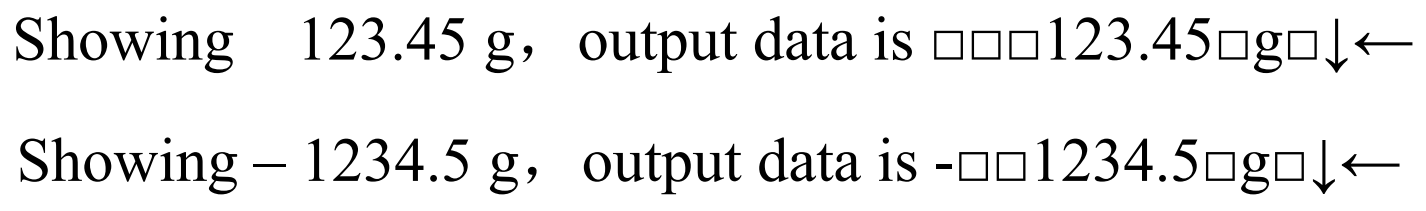
\includegraphics[scale=0.5]{obrazky/příklad protokolu - váha.PNG}
%    \end{center}
%    \label{priklad}
%    \caption{Příklad jak jsou data z displeje zapsány v datovém formátu \cite{vaha_datasheed}}
%\end{figure}



%Výstup reprezentovaný jako kod ASCII

%kombinace /r/n se vy uživa u WIndowsu k odřadkování pro 


%Vstupním portem je USB (viz. kapitola č. x), kdy piny

\section{Displej}
Další komponentou je displej, který je připojen k mikrokontroléru a zobrazuje název aktuálně měřeného destilátu, zůstatkový objem kapaliny v láhvi, maximální objem láhve, procento alkoholu měřeného destilátu a jeho obrázek pro případ, že by výrobce změnil tvar lahve, ale EAN kód by zůstal stejný.

\subsection{Požadavky na displej}
Hlavní požadavky na displej jsou:
\begin{itemize}
    \item Dotykový displej - pro budoucí implementaci klávesnice do displeje z důvodu redukce počtu periferií a snadnějšímu uživatelskému ovládání
    \item Uhlopříčka 5 - 7 palců (12,7 - 17,78 cm) pro dobrou čitelnost
    \item Bez rámečků s montážními otvory - možnost displej uchytit k vlastnímu rámu 
\end{itemize}

\subsection{Výběr displeje}

Vybraný displej je JOY-IT RASPBERRY PI touch display 7". Jeho důležité parametry jsou v tabulce č. \ref{displeej}\\

\begin{table}[!h]
    \centering
    \begin{tabular}{|c|c|}
        \hline
        Výrobce                                                         & JOY-IT   \\ \hline
        Uhlopříčka                                                      & 7" (17,78 cm)  \\ \hline
        Rozlišení                                                        & 1024 × 600 px    \\ \hline
         Rozhraní 
            & HDMI, USB \\ \hline
        Napájení & 5 V (0,6 A) \\ \hline
        Spotřeba & 3 W \\ \hline
        Dotykový displej                                                        & Ano     \\ \hline
        Cena                                                            & 2297 Kč     \\ \hline
    \end{tabular}
    \caption{Základní parametry vybraného displeje}
    \label{displeej}
\end{table}



\begin{figure}[!h]
    \begin{center}
        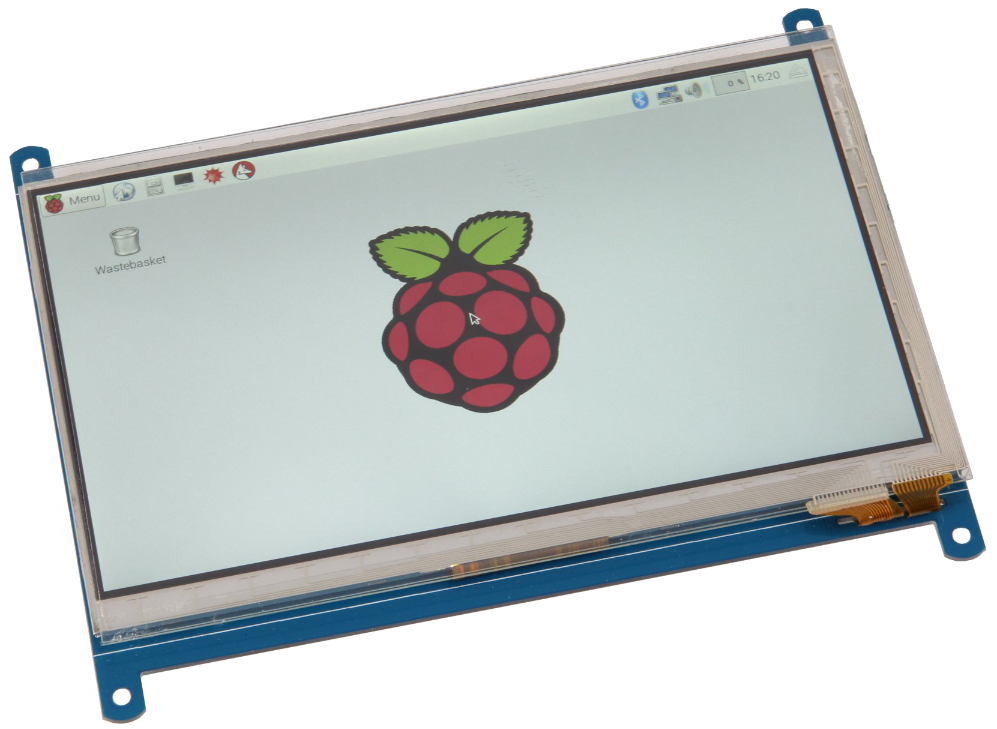
\includegraphics[scale=0.22]{obrazky/Displej.png}
    \end{center}
    \caption{Vybraný displej JOY-IT \cite{displej}}
\end{figure}

\subsection{Alternativy vybraného displeje}
Mezi alternativy můžeme zařadit:
\begin{itemize}
    \item JOY-IT RASPBERRY PI touch display 5"
    \begin{itemize}
        \item Uhlopříčka 5" (12,7 cm)
        \item Rozlišení 800x480 px
        \item Cena 1599 Kč
    \end{itemize}
    \item Raspberry Pi LCD - 7" Touchscreen
    \begin{itemize}
        \item Uhlopříčka 7" (17,78 cm)
        \item Rozlišení 800x480 px
        \item Cena 1399 Kč
        \item Horší dostupnost na českém trhu.
    \end{itemize}


    \item JOY-IT RASPBERRY PI touch display 5" - displej se liší od vybraného menší uhlopříčkou(5"), menším rozlišením(800x480) a nižší cenou(1599 Kč)
    \item Raspberry Pi LCD - 7" Touchscreen - displej se liší od vybraného menším rozlišením(800x480) a nižší cenou(1399 Kč). Jeho nevýhodou je horší dostupnost na českém trhu
\end{itemize}

%Displej je připojen k mikrokontroleru
%Displej nám bude zobrazovat data o 

\section{Čtečka čárového kódu}
Čtečka čárového kódu je zařízení, které, jak jeho název napovídá, umí číst grafický kód skládající se z černých a bílých proužků různých šířek, které reprezentují čísla splňující určitý standard pro obchodní průmysl, jako je například formát EAN. EAN (European Article Number) je mezinárodní unikátní identifikační číslo, které usnadňuje prodejcům prodej zboží. Pro český trh se běžně využívá EAN-13 (13-ti místné číslo nacházející se pod čárovým kódem). 

Čárové kódy se dělí na jednorozměrné (1D, lineární), které běžně známe z produktů v obchodech (černobílé proužky) a dvojrozměrné (2D) reprezentované jako matice bodů. Nejznámějším 2D formátem je QR (Quick Response) kod, který se využívá k rychlému placení, sdílení URL adres, připojení k internetu, atd. V praxi jsou 1D kódy, uloženy v databázi obchodu, ke kterému je přiřazen název a cena produktu.
%Čtečka čárového kódu je zařízení, které, jak jeho název napovídá, umí číst kód skládající se z černých proužků různých délek \cite{carovy_kod}, které reprezentují čísla splňující EAN standard.
%zdroj1: https://pageloot.com/cs/carovy-kod/jak-funguje-skener-carovych-kodu/
%zdroj2: https://cs.wikipedia.org/wiki/%C4%8Cte%C4%8Dka_%C4%8D%C3%A1rov%C3%A9ho_k%C3%B3du

%EAN (European Article Number) je mezinárodní unikátní identifikační číslo, které usnadňuje prodejcům prodej zboží. Pro český trh se běžně využívá EAN-13 (13-ti místné číslo nacházející se nad čárovým kódem) \cite{EAN}
%zdroj: https://cs.wikipedia.org/wiki/European_Article_Number

%V praxi je toto číslo uloženo v databázi obchodu, které je spojeno s název produktu a jeho cenou. Po načtení čárového kódu. %Po načtení čárového kódu

%V praxi je toto číslo uloženo v databázi obchodu, ke kterému je přiřazen název a cena produktu.

%Každé zboží se dá lehce indetifikovat pomocí

%V této sekci se nebudeme zabývat, jakým způsobem jsou čísla kódována do této podoby, ale jakým způsobem lze tyto čárové kódy číst.

Čárový kód se skládá z ochranných znaků „start“ a „stop“, ze středového dělícího znaku a z datových znaků, které reprezentují jednotlivé číslice. Formát EAN‑13 konkrétně určuje, že první tři číslice (tzv. prefix) značí zemi nebo region registrace, následujících šest jich slouží k identifikaci výrobce a dalších pět k rozlišení konkrétního produktu. Poslední třináctá číslice má kontrolní charakter. Vypočteme ji tak, že od konce kódu sčítáme číslice (kontrolní číslici ignorujeme) na lichých pozicích (1., 3., 5. atd.). Získaný součet vynásobíme trojkou, potom přičteme součet číslic, které leží na sudých pozicích. Výsledné číslo odečteme od nejbližšího vyššího násobku deseti a takto získaný rozdíl je kontrolní číslice. Tento postup pomáhá ověřit správnost EAN‑13 a minimalizuje chyby při skenování. [zdroj1][zdroj2]
%Zdroj1: https://is.ambis.cz/th/jmeqf/BP_Carove_kody_MMachan_3BK_IT.pdf
%Zdroj2: https://www.vut.cz/www_base/zav_prace_soubor_verejne.php?file_id=16877

\begin{figure}[!h]
    \begin{center}
        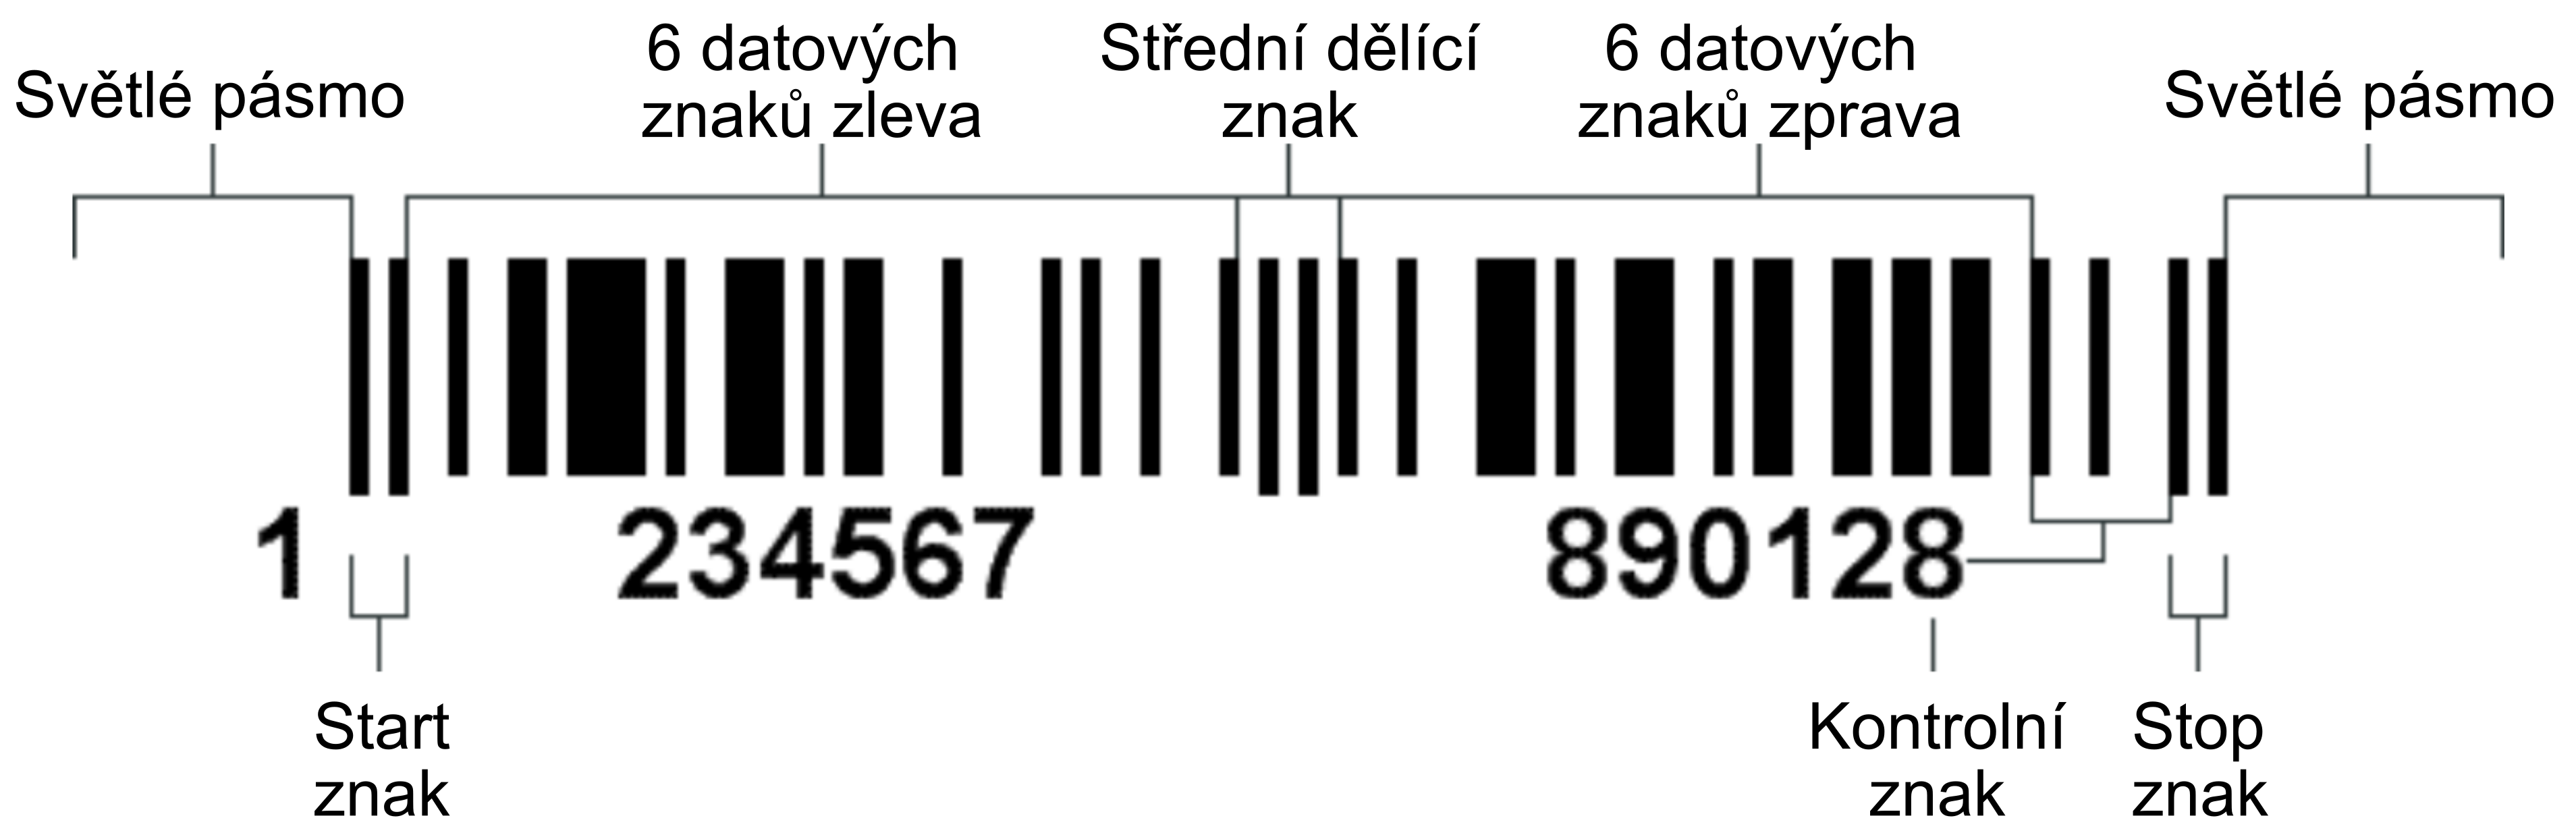
\includegraphics[scale=0.15]{obrazky/čárový kód.png} %0.5
    \end{center}
    \caption{Ukázka čárového kódu EAN-13.}
    \label{čárový kod}
\end{figure}





\subsection{Požadavky na čtečku čárového kódu}
Na trhu existuje celá řada čteček lišících se přesností, způsobem implementace a velikostí. Pro navrhovaný systém je vyžadována čtečka bez ochranného krytu s montážními otvory nebo s dostatečným prostorem pro jejich vyvrtání, aby čtečku bylo možné integrovat do vlastní konstrukce (krabičky) společně se všemi dalšími komponenty. Přednost se dává technologii CCD nebo kamerovému snímači díky vyšší mechanické odolnosti (např. při pádu) a lepší čitelnosti částečně poškozených kódů.
V poslední řadě je nutné, aby čtečka zvládala číst EAN-13 a méně často používaný EAN-8.

%dodelat zde tabulku: technologie: Kamerove (cmos), typ kodu: 1D, 2D, rychlost čtení, proudový odběr


%Na trhu je dostupných více druhů senzorů, které se liší požadavky na přesnost, druh implementace, velikostí atd. Velikost se požaduje menší bez ochranné krabičky pro budoucí uchycení do navrhnuté krabičky, která zastřeší všechny komponenty systému na jednom místě. včetně montážních otvorů nebo dostatečného prostoru pro jejich vyvrtání. Preferovanou technologií je CCD nebo CMOS z důvodu větší durability např. při pádu měřícího systému na zem a lepší čitelnosi poškozených kódů. Navíc od roku 2025 by mělo z obchodník řetězců vymizet klasické 1D čárové kódy a měli by je nahradit 2D QR kody, otázkou je zda přibude i nový formát 2D kódů na kterou budou vyvýjeny nové čtecí systémy

%Požaduje se komunikační rozhraní, nejlépe USB nebo UART pro odesílání a přijímání dat ze čtečky. Datový formát nejlépe ASCII, stejně jako u vybrané váhy, pro jeho jednoduché zpracování.

%Komunikační rozhraní čtečky se požaduje UART nebo USB s možností povolení virtuálního seriového portu pro komunikaci s mikrokontrolérem - označováno USB VCom.

%Další požadavek spočívá v tom, aby čtečka byla schopna číst standard EAN-13, který je běžně používán v České republice, a také EAN-8, s nímž se lze výjimečně setkat.
\subsection{Vybraná čtečka čárového kódu}

%Vybraná čtečka je GM65 od společnosti KROW, využívající CMOS technologie, obrázek č.\ref{gm65}.
%Čtečka disponuje UART a USB VCom. Kompletní specifikace je obsažena v dokumentaci.\cite{scaner}
%Datový formát pro seriovou komuniaci čtečky je stejný jak u vybrané váhy[xx] i zde chybý ověřovací bit, který bude ošetřen softwarově

%Z důvodu technologického pokroku a podle výše zmíněných parametrů jsem byl schopen najít pouze CMOS čtečky, proto tedy vybraná čtečka je GM65....

S ohledem na výše uvedené požadavky byla vybrána kamerová čtečka KROW GM65, využívající optických snímačů CMOS (viz obrázek č.\ref{gm65}) a LED diody pro nasvícení čárového kódu v hůře osvětleném prostředí. Čtečka nabízí komunikační rozhraní UART a USB. Datový formát pro sériovou komunikaci je shodný s vybranou váhou [\ref{datový paket váhy}].
%Podobně jako u váhy chybí ověřovací bit, který bude řešen softwarově. Podrobné technické specifikace čtečky jsou uvedeny v její dokumentaci.

\begin{table}[!h]
    \centering
    \begin{tabular}{|c|c|}
        \hline
        Výrobce                & KROW             \\ \hline
        Model                  & GM65             \\ \hline
        Typ                    & Kamerová čtečka  \\ \hline
        Čtecí vzdálenost \tablefootnote{Pro standart EAN-13 s šířkou kódu 35,6 mm při intenzitě osvětlení 250 lux}       & 4 - 25 cm            \\ \hline
        Rozhraní & HDMI, USB \\ \hline
        Napájení               & 5 V (až 160 mA)  \\ \hline
        Spotřeba               & 0,8 W            \\ \hline
        Rychlost čtení         & 0,1 s            \\ \hline
        Cena                   & 992 Kč           \\ \hline
    \end{tabular}
    \caption{Základní parametry vybraného displeje}
    \label{displeej}
\end{table}


\begin{figure}[!h]
    \begin{center}
        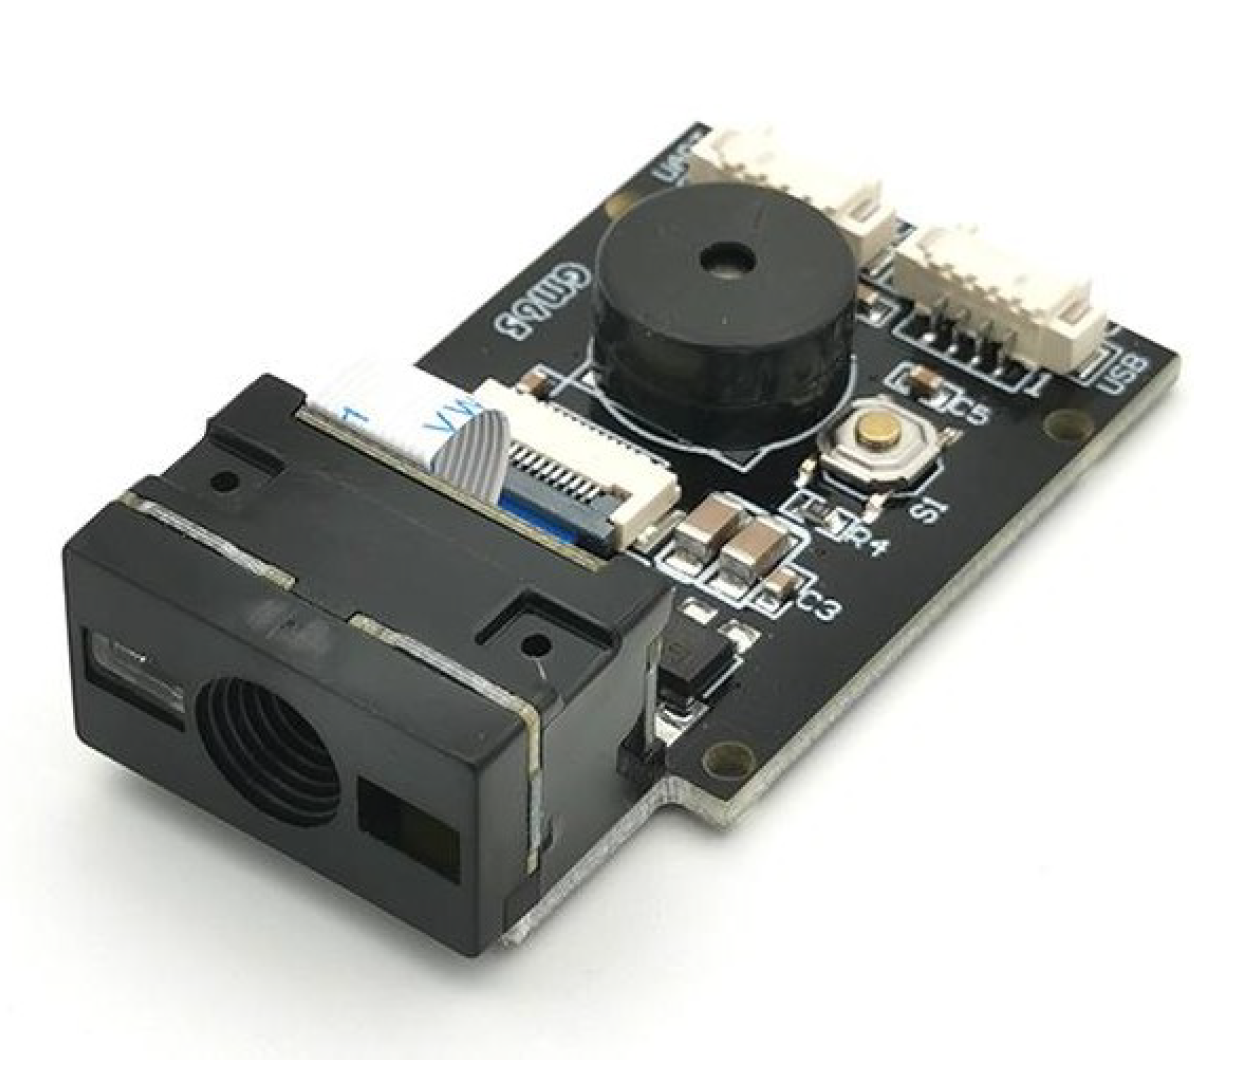
\includegraphics[scale=0.25]{obrazky/gm65.PNG} %0.5
    \end{center}
    \caption{Vybraná čtečka čárového kódu KROW GM65 \cite{scaner}}
    \label{gm65}
\end{figure}

%Toto níže je blbost
%\begin{table} [!h]
%    \centering
%    \begin{tabular}{|l|l|l|l|l|l|}
%    \hline
%         Hlavička  & Typ & Délka dat & Adresa & Data & CRC \\ \hline
%         2 B       & 1 B & 7 B       & 3    B & 1 B  & 1 B\\ \hline 
%    \end{tabular}
%    \caption{Předpis výstupních dat}
%    \label{datovy format čtečky}
%\end{table}




\subsection{Alternativy vybrané čtečky čárového kódu}
%Mezi alternativy můžeme zařadit:
%Vybrané alternativy jsou kamerové

\begin{itemize}
    \item YHDAA YHD-M800D
    \begin{itemize}
        \item Typ: Kamerový snímač
        \item Cena: 1000 Kč
        \item Rozhraní: USB
        \item Nepřehledná a nevypovídající dokumentace
    \end{itemize}
    \item WaveShare Barcode Scanner
    \begin{itemize}
        \item Typ: Kamerový snímač
        \item Cena: 1318 Kč
        \item Rozhraní: USB, UART
    \end{itemize}
\end{itemize}


%\begin{itemize}
  %  \item YHDAA YHD-M800D - kamerová čtečka, cenově stejně dostupné(1000 Kč) jak vybraná čtečka, integrovaný USB port, nepřehledná a nevypovídající dokumentace 
 %   \item WaveShare Barcode Scanner - kamerová čtečka, dražší než vybraná čtečka(1318 Kč), integrovaný sériový port micro USB a UART
%\end{itemize}

\section{Modul s výpočetní jednotkou} %Mikrokontroler
%Výpočetní modul / Modul s výpočetní jednotkou / Řídící jednotka / Výpočetní jednotka

Modul s výpočetní jednotkou je samostatná hardwarová součást (obvykle deska plošných spojů osazená procesorem, pamětí a potřebnými rozhraními), která ve větším elektronickém či řídicím systému zajišťuje hlavní výpočetní výkon. Často pracuje v kombinaci s jinými moduly – sběrnicovými, vstupními (senzory, klávesnice), výstupními (displeje, motory) nebo dalšími výpočetními jednotkami. Mezi běžné představitele těchto výpočetních jednotek patří:
\begin{itemize}
    \item Mikrokontrolery (Jednočipové PC, MCU): Jsou to systémy na jednom čipu, které integrují procesor, paměť flash a RAM, A/D převodník, oscilátor (hodiny) a I/O porty. Běžně se využívají v real-time aplikacích, jež nevyžadují vysoký výpočetní výkon.
    \item Jednodeskové počítače (SBC, mikropočítače): Vyšší stupeň integrace oproti mikrokontrolérům. Jde o plnohodnotné počítače na jedné desce. Obvykle běží pod operačním systémem a nabízejí více periferií, což je činí vhodnými pro komplexní a výpočetně náročnější úlohy.
\end{itemize}


%Mikrokontroler jinak označovaný jednočipový počítač je integrovaný obvod
%Mikrokontrolér nebo také jednočipový počítač je integrovaný obvod obsahující kompletní mikropočítač. Jednočipové počítače se vyznačují velkou spolehlivostí a kompaktností, proto jsou určeny především pro jednoúčelové aplikace. Mikrokontroléry jsou často používány v embedded systémech, jako jsou například řídicí systémy, regulátory, senzory a další aplikace, kde je potřeba rychle a spolehlivě zpracovávat data. V praxi si můžeme pod takovou řídící jednotkou představit např. PLC (Programovatelný automat)
%[zdroj]
%Na bakalařku překopat...je to opsaný
%https://sk.wikipedia.org/wiki/Mikrokontrol%C3%A9r
%https://cs.wikipedia.org/wiki/Jedno%C4%8Dipov%C3%BD_po%C4%8D%C3%ADta%C4%8D

\subsection{Požadavky na modul s výpočetní jednotkou} %Požadavky na řídící jednotku / výpočetní modul
%napájení
%OS(bez os nepojede databaze atd) a grafická čip, hdmi,  pro vývoj GUI
%Jednodeskotopový PC skrz chod pythonu a Tkinter, ten na mikrokontroleru nerozjedu skrz malou pamět a výkon a na MikroPython nic takového nebude. Dále mikrokontorler nemá SD slot pro ukládání databáze
%V mobilu mam napsany od petyho proč nevybrat to a tam a nejaky popis k mikrokontrolerum

%

Hlavním z požadavků je snadná realizovatelnost firmware s integrovaným grafickým uživatelským rozhraním(GUI) ovládaného dotykovým displejem. Pro takové účely je vhodné použít vysokoúrovňový programovací jazyk, např. Python, který nabízí široký výběr knihoven a nástrojů, které ulehčují a zrychlují vývoj samotného firmware, na druhou stranu je nutné přihlédnout na dostačující výkon a operační paměť(RAM) řídící jednotky. Vývoj GUI a práce s databází obnáší zpravidla přítomnost OS už jen z důvodu zabudovaných grafických ovladačů pro komunikaci s displejem, správu paměti nebo využití grafických knihoven, které je pro svoji funkčnost OS vyžadují, proto využiji nenáročné distribuce linuxu, která je oproti konkurenčním OS výkonově i paměťově nenáročná.
%Z důvodu volby vysokoúrovňového programovacího jazyku, GUI a využití databáze je nutné, aby firmware běžel na OS.
%Z důvodu minimální výkonové a paměťové náročnosti poběží řídící jednotka na nenáročné distribuci Linuxu. Pro takový účely se hodí libovolná distribuce linuxu, která je hojně využívána u jednodeskových počítačů.

Další požadavky:
\begin{itemize}
    \item Výkon a paměť: 
        \begin{itemize}
            \item Dvou a více jádrový procesor pro paralelní chod GUI a stavového automatu pro zpracování dat ze čtečky čárového kódu a váhy. 
            \item Minimální velikost RAM paměti 2 GB, optimálně 4-8 GB pro plynulý chod GUI a OS.
        \end{itemize}
    \item Periferie:
        \begin{itemize}
            \item 3x USB-A(optimálně verze 3.0) pro čtečku čárového kódu, váhu a napájení displeje. Výstupní proud alespoň 0,6 A 
            \item 1x HDMI nebo Micro HDMI pro dotykový displej
            \item slot na SD kartu na které budou uložena veškerá data databáze zmíněná v kapitole č. 5.3, operační systém a samotný firmware. Velikost SD karty alespoň 32 GB[zdroj1] pro plynulý chod OS  
            %pro optimální rychlost čtení a zápisu [zdroj1][zdroj2]. %Například pro Rasbian OS (OS jednodeskových počítačů(SBC) raspberry pi) je doporučovaná velikost minimálně 4 GB[Zdroj1]
            %Zdroj1 : https://www.raspberrypi.com/documentation/computers/getting-started.html
            %Zdroj2 : https://www.raspberrypi.com/documentation/accessories/sd-cards.html
            \item Řídící jednotka musí zvládnout poskytnout dle vybraných komponent, alespoň 0,7 A při 5 V, optimálně 1,2 A, pro případ rozšíření systému o další komponenty.
            %\item Alespoň jeden GPIO pro ovládání pípáku
        \end{itemize}
    \item Integrovaný Wi-Fi modul: Do budoucna je cílem bezdrátová konektivita s měřícím systémem pomocí mobilní aplikace nebo připojení k ERP systémům
    %\item napájení/odběr/příkon/spotřeba: ...
    %Výstupní proud 0,6 A (USB): Výkonově nejnáročnější komponentou připojené k řídící jednotce bude displej[] s proudovým odběr 0,6 A při 5 V. (Do budoucna bude měřicí systém bude obsahovat baterii, který může napájet jednotlivé komponenty.) Pro provoz displeje, který je proudově nejnáročnější je nutné, aby USB porty dokázaly poskytnout minimálně 0,6 A při 5 V. Řídící jednotka musí zvládnout poskytnout dle vybraných komponent, alespoň 0,7 A při 5 V, optimálně 1,2 A, pro případ rozšíření systému o další komponentu.
\end{itemize}

%Nevybírat model s konrétní velikost ram, ale určit více velikostí a pak podle toho dát rozsah ceny
\subsection{Vybraný modul s výpočetní jednotkou}
Na základě výše zmíněných požadavků byl vybrán jednodeskový počítač Raspberry Pi 4 ve verzi s 4 GB operační paměti. Kategorii mikrokontrolérů jsem úplně vynechal z důvodu nedostatečného výkonu a operační paměti pro chod OS s GUI aplikací a absence integrovaných periférií jako USB nebo HDMI. 

Mezi klíčové výhody Raspberry Pi patří široká komunita, kvalitní podpora i bohatá škála dokumentace a knihoven. Další z výhod je rozumný poměr cena výkon a spolehlivost. Základní technické parametry jsou přehledně uvedeny v tabulce č. \ref{raspbericko_spec}, zatímco kompletní specifikace lze nalézt v příslušné dokumentaci. \cite{Raspberry pi}

%Vyrobce
%Model
%Procesor
%RAM
%Rozhraní 2x USB 2.0, 2x USB 3.0, 2x HDMI 1.4 (asi)
%Napájení 5V DC
%Spotřeba 4 - 7 W
%Dále obsahuje: Wi-Fi/BT modul, SD slot, 3,5 mm Jack


\begin{table}[!h]
    \centering
    \begin{tabular}{|c|c|}
        \hline
        Výrobce                                                         & Raspberry Pi Foundation   \\ \hline
        Model                                                           & Raspberry Pi 4  \\ \hline
        %\begin{tabular}[c]{@{}c@{}}Komunikační\\ protokol\end{tabular}  & UART   \\ \hline
        CPU & \begin{tabular}[c]{@{}c@{}}1.5GHz čtyřjádrový \\ ARM Cortex-A72\end{tabular} \\ \hline
        GPU & VideoCore VI 500 MHz \\ \hline
        RAM & 4 GB \\ \hline
        Periferie & \begin{tabular}[c]{@{}c@{}} 2x USB-A 3.0 \\ 2x USB-A 2.0 \\ 1x USB-C (napájení) \\ 2x microHDMI 2.0 \\ 1x Gigabit Ethernet \\ 40x GPIO \end{tabular} \\ \hline
        Napájení                                                        & 5 V DC (až 3 A)   \\ \hline
        Spotřeba                                                        & 3 - 7 W     \\ \hline
        Dale obsahuje & \begin{tabular}[c]{@{}c@{}} Wi-Fi/BT modul \\ SD slot \end{tabular} \\ \hline
        Cena                                                            & 1987 Kč     \\ \hline
    \end{tabular}
    \label{raspbericko_spec}
    \caption{Základní parametry Raspberry Pi 4 \cite{Raspberry pi}}
\end{table}

%Hlavní nevýhodou je pořizovací cena 1479 Kč a vyšší spotřeba energie v rozmezí 3 - 7 W. Kompletní specifikace se nachází v dokumentaci výrobce.[2]



%Vybraný mikrokontroler byl Raspberry PI 4, který dokáže pokrýt veškeré požadavky na měřicí systém. Konkrétně se jedná o model B s 4 GB operační paměti. Zde jsou zmíněné požadavky na mikrokontrolér:

%\begin{itemize}
%    \item Dostatečný počet portů pro připojení všech modulů.
%    \item Integrovaná čtečka SD karty pro ukládání databáze
%    \item Dostatečný výkon pro chod GUI aplikací. Do budoucna je v plánu implementovat dotykový displej, na kterém budou veškeré informace pěkně přehledné díky grafickému rozhraní
%    \item Integrovaný čip pro bezdrátovou konektivitu. Do budoucna možnost vývoje mobilní aplikace k vyvíjenému systému nebo bezdrátové připojení k ERP systémům.
%    \item
%    \item Hlavní z požadavků je snadná realizovatelnost firmware s integrovaným grafickým uživatelským rozhraním pro ovládání dotykového displeje. Pro takový účely je vhodné použít programovací jazyk Python, který nabízí širší výběr knihoven a nástrojů, které ulehčují a zrychlují vývoj samotného firmware.
%
%    \item
%\end{itemize}
%Dost požadavků je nad rámec bakalářské práce, ale pro budoucí inovaci systému nemusíme měnit mikrokontrolér a realizovat znovu už fungující HW kompatibilitu mezi komponenty a vyvíjet SW vybavení.

%Jedinou nevýhodou je vysoká pořizovací cena.

\begin{figure}[!h]
    \begin{center}
        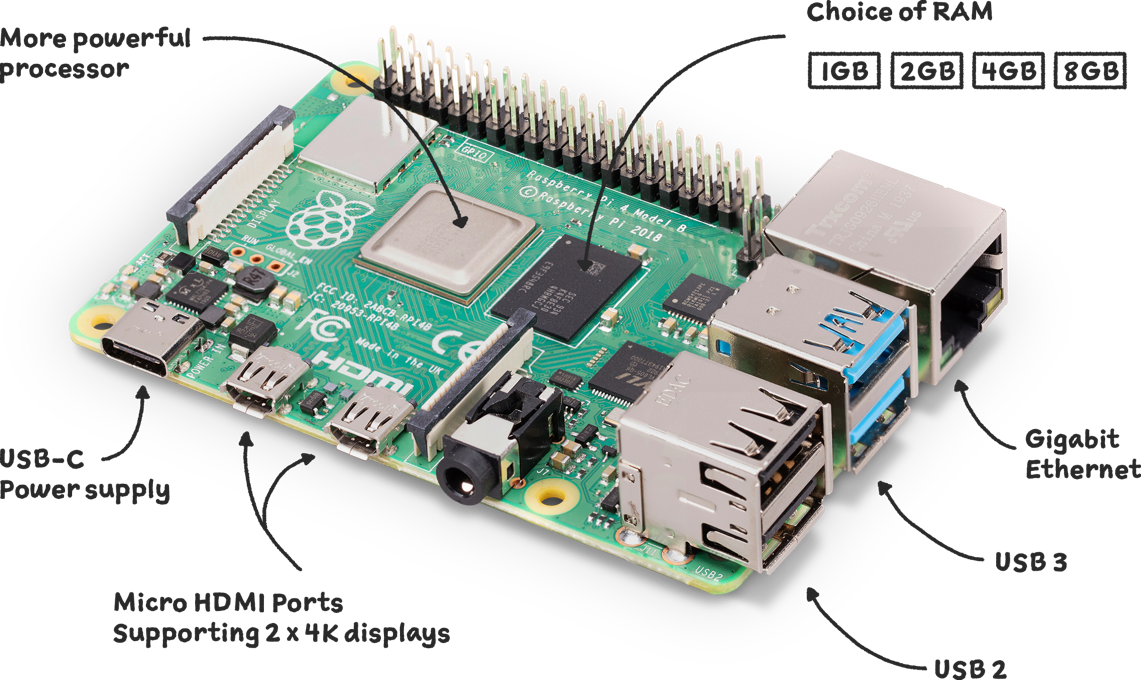
\includegraphics[scale=0.3]{obrazky/raspberry-pi-4.png}
    \end{center}
    \caption{Vybraný jednodeskový PC Raspberry Pi 4 \cite{malina_obr}}
    %\label{gm65}
\end{figure}

\subsection{Alternativy vybraného modulu s výpočetní jednotkou}

%Raspberry piko
%Arduino Uno
%Esp 32 (SoC/mikrokontroler + WIFI/BT)
%Acemagic T8-PRO N5105 (8+0) Silver (Přebustěny jednodeskový pc / mini PC)

\begin{itemize}
    \item ESP32 (MCU)
        \begin{itemize}
            \item Zlomová cena - 200 Kč
            \item Absence debuggeru
            \item ...
        \end{itemize}
    \item Banana Pi M5 (Druhá nejlepší volba)
        \begin{itemize}
            \item[$-$] "Čínská" kopie raspberry pi 4
            \item[$+$] Výkonnější procesor - Cortex-A55 (4 jádra, 2 GHz)
            \item[$+$] Integrované uložiště eMMC (rychlejší než SD karta)
            \item[$-$] Horší dostupnost v lokálních e-shopech (často nutný dovoz)
            \item[$-$] Menší uživatelská základna - méně zdrojů, tutoriálů a komunitních projektů
            \item[$+$] 2000 Kč
        \end{itemize}
    \item Odroid XU4
        \begin{itemize}
            \item[$-$] Absence Wi-Fi modulu
            \item[$-$] Pouze 2 GB RAM
            \item[+] eMMC modul
            \item[$+$] Komunita kolem Hardkernel Odroidů je relativně aktivní
            \item[$-$] Stále menší komunita než u Raspberry
        \end{itemize}
    %- Jen 2 GB RAM. Nemá integrovaný Wi-Fi modul, nutnost připojit externě.
    \item NVIDIA Jetson Nano 
        \begin{itemize}
            \item[$-$] Cenově náročný - 8000 Kč
            \item[$+$] Zbytečně vysoký grafický výkon. Vhodnější spíše pro strojové učení a práci s AI.
            \item[$-$] Absence Wi-Fi modulu (možnost externího připojení)
            \item[$-$] Vyšší spotřeba 7 - 24 W
        \end{itemize}
    \item Recyberry Asus Tinker Board S. 
        \begin{itemize}
            \item[$-$] Aktuálně nedostupný na českém trhu%Horší dostupnost v lokálních e-shopech
            \item[$-$] Operační paměť max. 2 GB
            \item[$-$] Pouze USB 2.0 (10x pomalejší než USB 3.0 %[zdroj: to co useriove komunikace])
            \item[+] Integrovaný eMMC (rychlejší načtení OS)
        \end{itemize}
    %\item Recyberry Asus Tinker Board 2S - Vyší napájecí napětí 12-19 V, 
    %\item Arduino Portenta X8 - Nemá nativní HDMI port, ale zde využít USB-C konektoru jako Displey Port a pro ostatní USB porty použít USB rozbočovač
\end{itemize}



%Rozhodoval jsem se mezi dalšími dvoumi 







%proč malinu:
%
%-graficky čip pro dotykovy displej, 
%
%-wifi/BT čip pro budouci mobilni aplikaci, 
%
%-možnost vývoje GUI (python, CS) bezne mikrokontrole funguje jen na C/C++ asi,
%
%-rozumně velké uložiště pro ("GUI aplikaci" spíš RAM) databázi, která se časem bude rozšiřovat nevim jestli by arduino to pojmulo, ale určitě arduino nepojme databází obrázků, jednotlivých destilátů
%%https://www.dps-az.cz/clanky/id:6173/uvod-do-embedded-systemu